\section{6LoWPAN implementation in \mbox{Mote Runner}}
\begin{frame}[fragile]
  \frametitle{Introduction to 6LoWPAN}
  \begin{figure}
    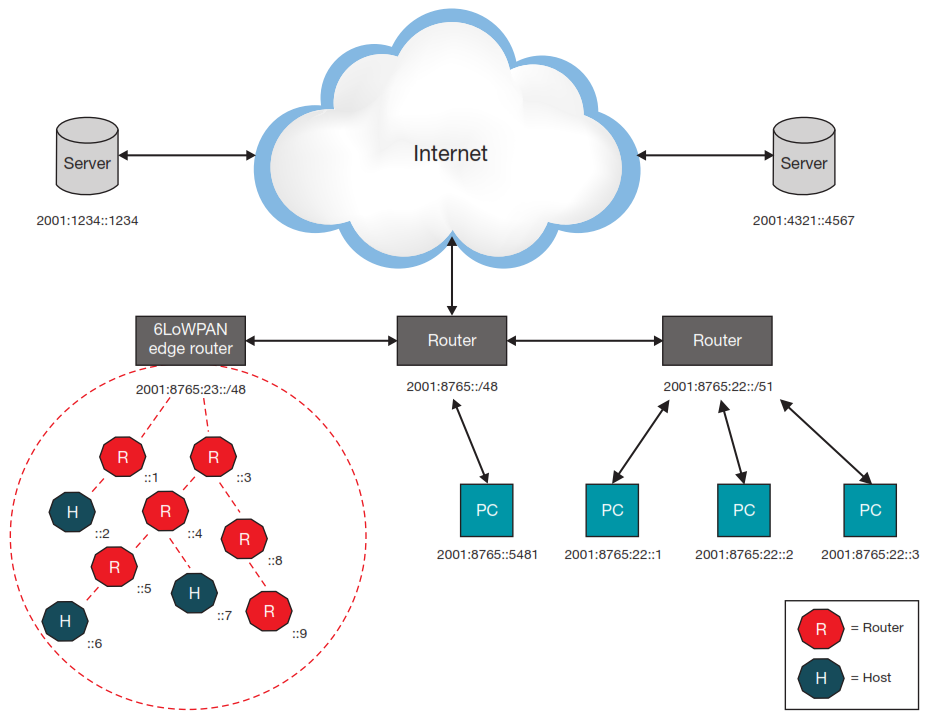
\includegraphics[width=.7\textwidth]{img/6low_network.png}
    \caption{IPv6 network with a 6LoWPAN mesh network}
  \end{figure}
\end{frame}

\begin{frame}[fragile]
  \frametitle{6LoWPAN stack}
  \begin{figure}
    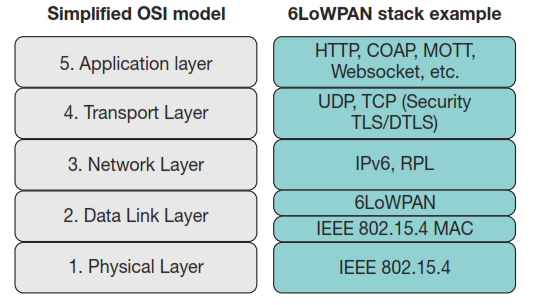
\includegraphics[width=.6\textwidth]{img/6low_stack.png}
  \end{figure}
\end{frame}

\begin{frame}[fragile]
  \frametitle{MRv6: an implementation of 6LoWPAN in MR}
  \begin{itemize}
    \item TDMA and beacon based multi-hop network which allows for an IPv6 based communication between motes
    \item It is not a built-in MR component, but it is fully implemented in C\#
    \item Datagram packets exchanged adheres to a subset of the 6LoWPAN specifications
    \item The edge mote decides upon:
    \begin{itemize}
      \item Association requests
      \item Assigns communication schedules between wireless nodes
      \item Determines the routes in the network
    \end{itemize}
  \end{itemize}
\end{frame}

\begin{frame}[fragile]
  \frametitle{MRv6: Limitations}
  \begin{itemize}
    \item Only the transmission of UDP packets within the 6LoWPAN network is supported
    \item Exists only a proprietary broadcast operation to reach all motes in the network
    \item Is not suited for low latency application
    \item Does not support packet segmentation, reassembly and flow control
    \item Has been deployed in 900MHz or 2.4GHz frequency ranges and uses a single channel in the 2.4GHz band yet
  \end{itemize}
\end{frame}

\begin{frame}[fragile]
  \frametitle{Scheduling}
  \begin{itemize}
    \item The network tree is only know to the edge
    \item The communication slots between parent and children are globally assigned by the edge and do never overlap
    \end{itemize}
    \begin{table}[h]
      \begin{tabular}{@{}|c|c|l|l|l|l|@{}}
	\toprule
	 SF edge & SF mote 1 & SF mote 2 & ... & SF max mote \\ \bottomrule
      \end{tabular}
    \end{table}
\end{frame}

\begin{frame}[fragile]
  \frametitle{Superframe}
  \begin{itemize}
   \item At the beginning of their communication period parent motes send out beacon messages
    \item Other then a fixed exclusive slot, parent offers a shared slot (e.g. association requests and responses, broadcast messages)
    \item Beacon, shared and fixed slots form the superframe whose timings are assigned by the edge
  \end{itemize}
  \begin{table}[h]
    \begin{tabular}{@{}|p{1.5cm}|p{1.5cm}|p{1.5cm}|p{1cm}|p{1.5cm}|p{1cm}|@{}}
      \toprule
      Beacon slot & Shared slot & Child slot 0 & ... & Child slot n & Gap \\ \bottomrule
    \end{tabular}
  \end{table}
\end{frame}

\begin{frame}[fragile]
  \frametitle{Association}
  \begin{itemize}
    \item The joining mote evaluates information in the beacons (e.g. number of children or hops to the edge)
    \item Mote sends and association request in the shared slot of the potential parent
    \item Parent forward the request to the edge with the EUI-64 of the joining mote
    \item When the edge accepts the mote:
    \begin{itemize}
      \item It allocates short address and superframe timings for the mote
      \item The parent forwards the response to the new child in its shared slot and adds it to its list
    \end{itemize}
  \end{itemize}
\end{frame}

\begin{frame}[fragile]
 \frametitle{Short comparison}
 \begin{table}[h]
    \begin{tabular}{@{}p{5cm}|p{5cm}@{}}
      \toprule
      Our Mac-Like &  MRv6 \\ \midrule
      Contention based &  Scheduled\\
      \hline
      Trasmitt only when  \mbox{requested} &  TDMA based\\
      Association managed by pan-coordinator & Association managed by the edge  \\ 
      ... & ... \\ \bottomrule
    \end{tabular}
  \end{table}
\end{frame}
